\documentclass[titlepage]{article}
\newcommand\tab[1][1cm]{\hspace*{#1}}
\usepackage[left=12mm, top=12mm, right=12mm, bottom=12mm]{geometry}
\usepackage{gensymb}
\usepackage{float}
\usepackage{graphicx}
\usepackage{subcaption}
\usepackage{hyperref}
\usepackage{forest}

\begin{document}

\title{COMP 4107 Final Project\\
         {\small Clean vs. Raw Data performance on an LSTM chatbot system}}
\author{Lachlan Campbell, 100999056\\
              Elijah MacPherson, 100970225}
\maketitle

\section{Introduction}
\tab For this project we will attempt to implement a chatbox trained off of various transcript datasets. We will accomplish this using recurrent neural networks communicating and learning via sequence to sequence learning. The object of this project is to determine the effects of the cleanliness of datasets have on the conversational accuracy as well as training time.

Two sets of input data were prepared from the movie dataset. The first was a `clean' version with punctuation and contractions removed. The second version of the input data was a `raw' version, with the cleaning and filtering turned off. For both sets of input data, sentences longer than 16 characters and shorter than 2 characters were removed.

\section{Background}
In order to implement this chatbot we will be using LSTM (Long short-term memory) neural networks.
\begin{figure}[H]
	\centering
	\captionsetup{justification=centering}
	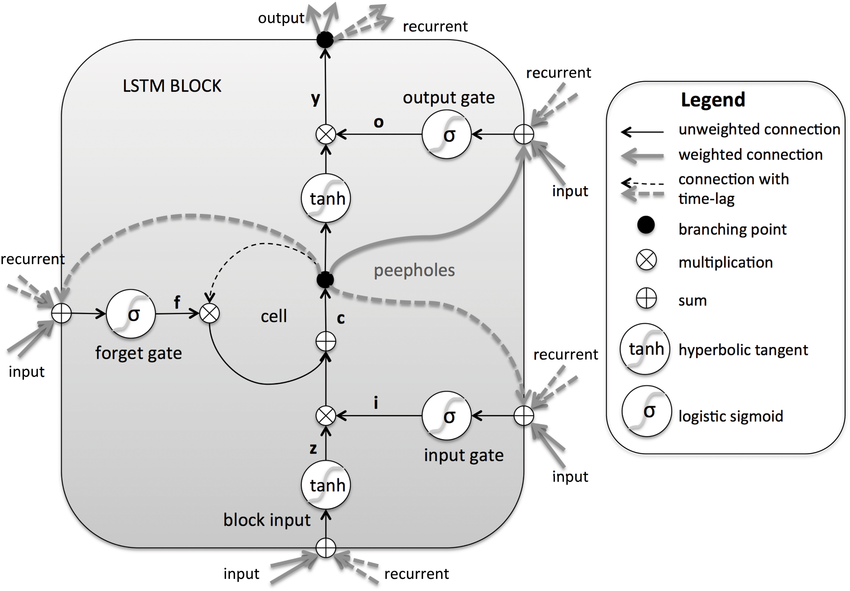
\includegraphics[width=120mm]{images/LSTM-model.png}
	\caption{An LSTM block recurrent neural network model. \\{\tiny \url{https://devblogs.nvidia.com/wp-content/uploads/2016/03/LSTM.png}}}
	\label{fig:lstm1}
\end{figure}
\begin{figure}[H]
	\centering
	\captionsetup{justification=centering}
	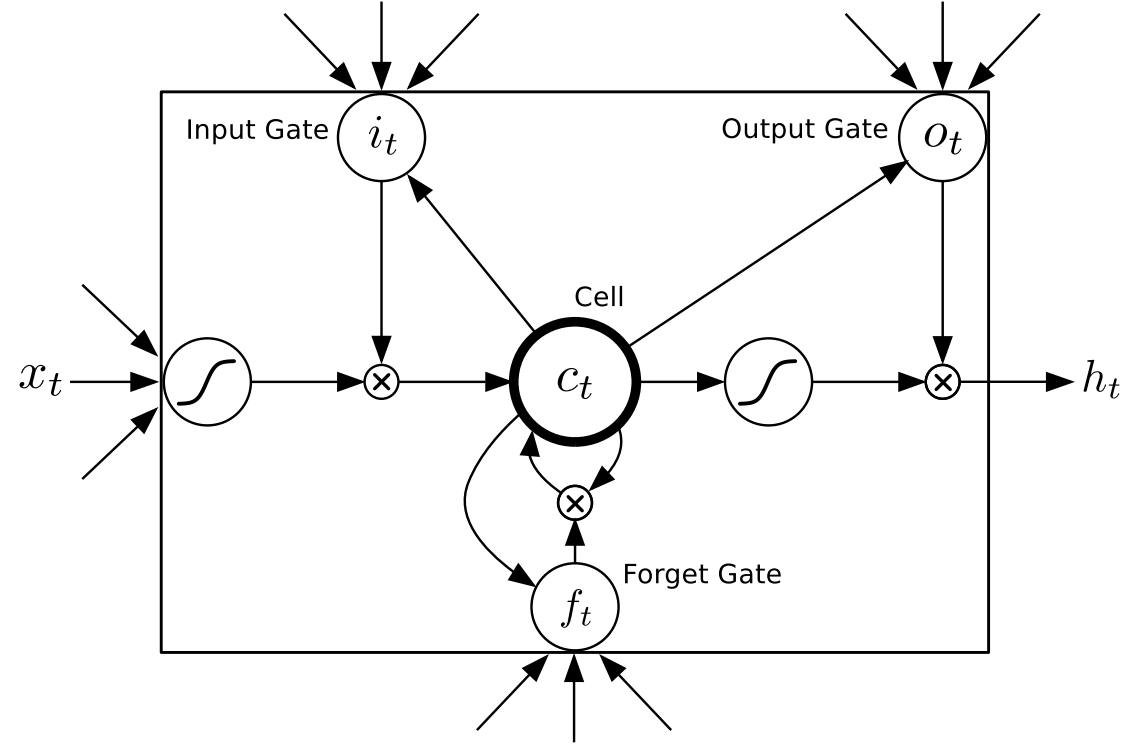
\includegraphics[width=120mm]{images/LSTM-model-2.png}
	\caption{A barebones view of the different gates involved in an LSTM.\\{\tiny \url{https://raw.githubusercontent.com/torch/torch.github.io/master/blog/\_posts/images/LSTM.png}}}
	\label{fig:lstm2}
\end{figure}
~\\~\\~\\~\\~\\	
\tab We will be using a method called sequence to sequence learning where two neural networks (namely an encoder NN and a decoder NN) communicate with each other in order to convert sequences from one domain to sequences in another domain. In our case we will be working within the domains of $statement\rightarrow reply$.
\begin{figure}[H]
	\centering
	\captionsetup{justification=centering}
	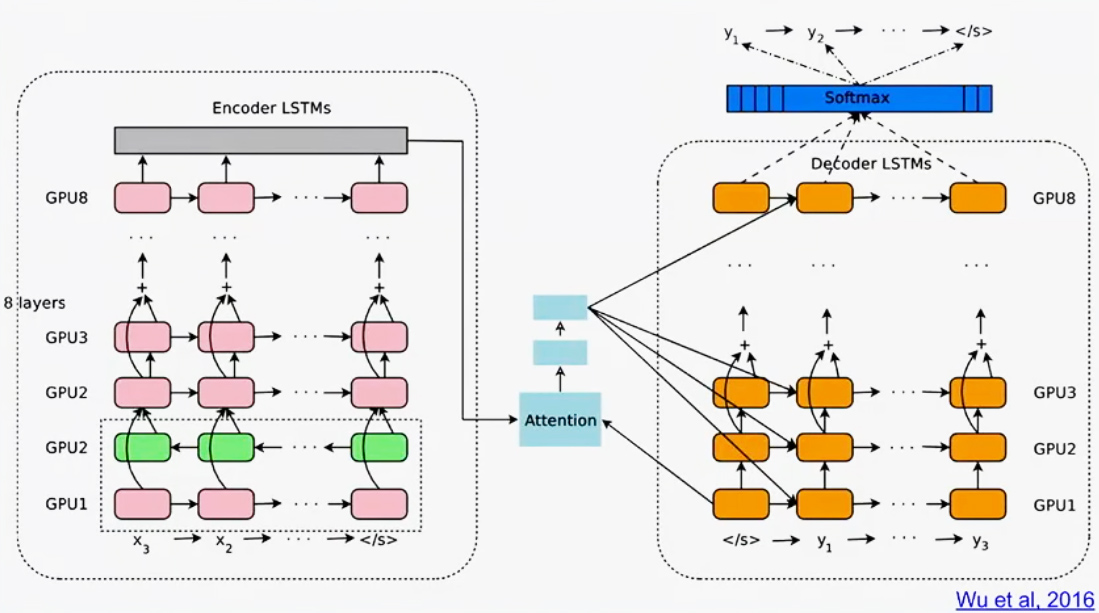
\includegraphics[width=120mm]{images/Seq2seq.jpg}
	\caption{A look at how google translate uses sequence to sequence learning to translate from one language to another. \\{\tiny \url{https://blog.altoros.com/wp-content/uploads/2017/04/tensorflow-dev-summit-2017-eugene-brevdo-keynote-sequence-models.jpg}}}
	\label{fig:seq2seqgoogletranslate}
\end{figure}
The model above uses many LSTM's in the encoder NN and the decoder NN, but for the purposes of the project we will only be using three LSTM's stacked in the encoder NN and one LSTM in the decoder NN.\\

\subsection*{The Dataset}
The dataset that was chosen was Cornell University's Movie Dialogue Corpus.\cite{chameleons, cornell} The dialogue corpus contains over 200,000 pieces of conversation between 10,292 movie characters in 617 movies. The dataset also includes metadata storing the genres, release year, IMDB rating and the number of IMDB votes for each movie. For each character, the metadata includes the gender and position on movie credits. This metadata was not used.

\section{Problem Statement}
The aim of this project is to determine what the effects of a cleaned data set are on the:\\
\tab 1. Training time of an LSTM chatbot network\\
\tab 2. Overall proficiency in training accuracy.

\section{Results and Analysis}
Before training can begin, let us first look at the computational graph of our model:
\begin{figure}[H]
	\centering
	\captionsetup{justification=centering}
	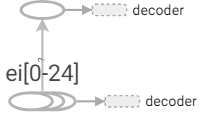
\includegraphics[width=80mm]{images/main_graph.png}
	\caption{The main graph of our chatbot network}
	\label{fig:maingraph}
\end{figure}
\begin{figure}[H]
	\centering
	\captionsetup{justification=centering}
	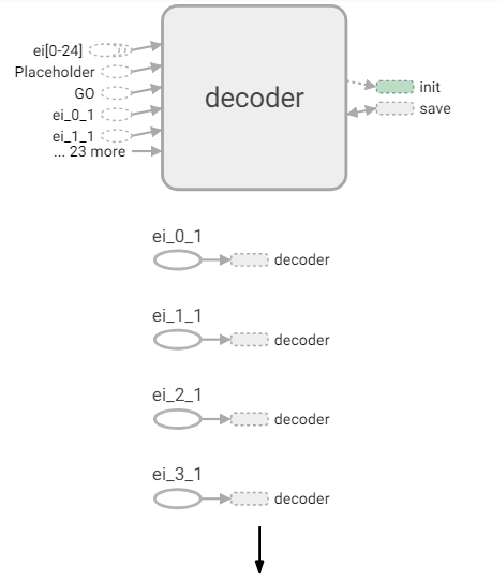
\includegraphics[width=100mm]{images/aux_nodes.png}
	\caption{A look at the auxilliary nodes of the model. Note there are 24 EI units in total.\\(extends below the arrow)}
	\label{fig:auxnodes}
\end{figure}

Training
\begin{figure}[H]
	\centering
	\begin{subfigure}[b]{0.4\linewidth}
		\centering
		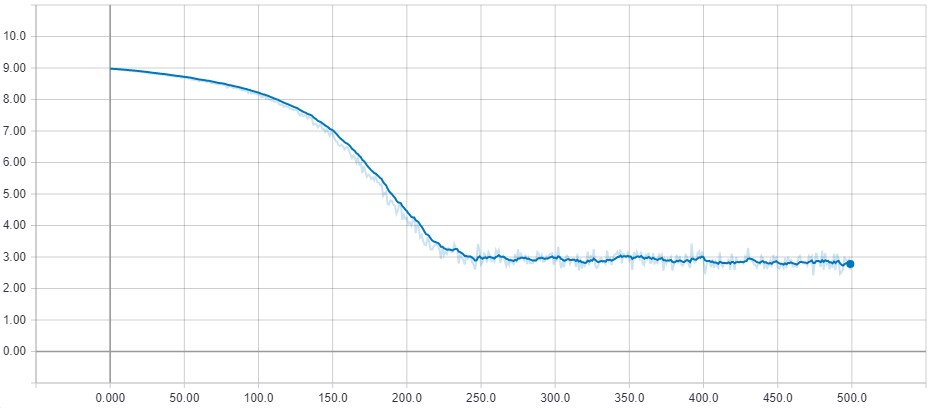
\includegraphics[width=\linewidth]{images/cost-clean-001.png}
		\caption{The cost function trained on a clean dataset\\with $\alpha = 0.001$}
	\end{subfigure}
	\begin{subfigure}[b]{0.4\linewidth}
		\centering
		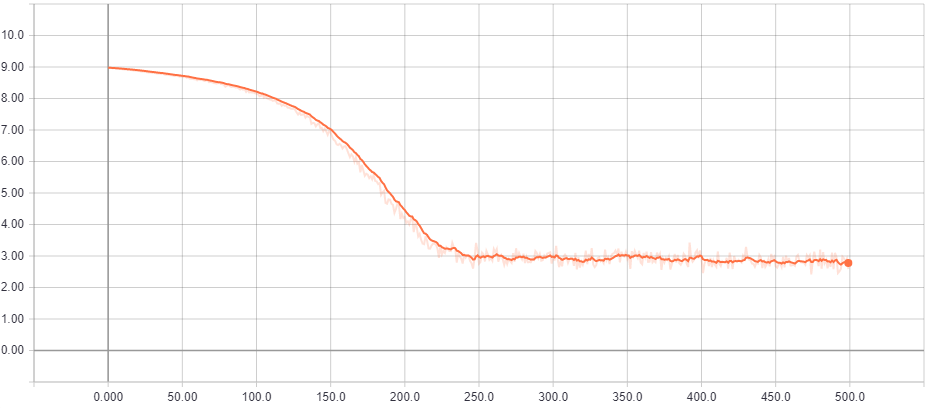
\includegraphics[width=\linewidth]{images/cost-raw-001.png}
		\caption{The cost function trained on a raw dataset\\with $\alpha = 0.001$}
	\end{subfigure}
	\label{fig:ccr001}
\end{figure}
As you can see from the graph the cost seems to settle around 250 epochs with a minimum value of approx. 2.7. If we overlay the two charts and remove the smoothing we get this:
\begin{figure}[H]
	\centering
	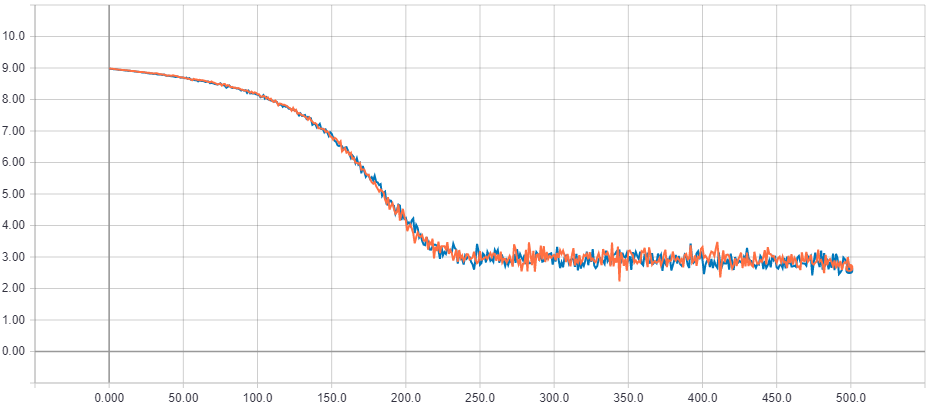
\includegraphics[width=120mm]{images/cost-overlap-001.png}
	\caption{Overlap of clean vs. raw dataset performance.}
	\label{fig:co001}
\end{figure}
As you can see from the graph there isn't much improvement in terms of actuall training accurracy with respect to the cleanliness of the dataset. They both converge in \textasciitilde 250 epochs, however if we switch the graphs to relative view, something interesting happens.
\begin{figure}[H]
	\centering
	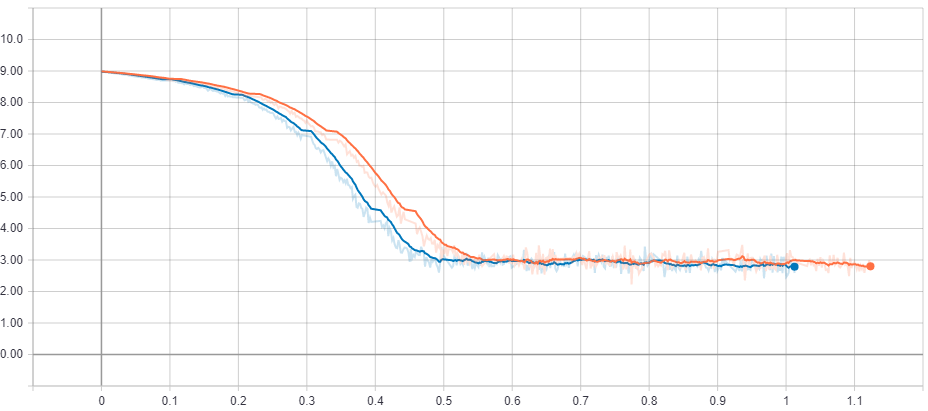
\includegraphics[width=120mm]{images/cost-overlap-relative-001.png}
	\caption{Overlap of clean vs. raw dataset with respect to training time.}
	\label{fig:cor001}
\end{figure} 
We can see from the figure above that the cleaned dataset takes about 5 minutes less to reach equilibrium. It also takes about 10 minutes less in order to reach 500 epochs. This is likely due to the fact that a clean dataset removes much of the verbosity out of the sentences, as well as unnecessary punctuation and overall longer or shorter sentances, so the network has a lot less fluff to deal with when training. 

\section{Conclusion}
It is clear that cleaning the dataset doesn't have much of an effect on the overall performance of the network in terms of training accuracy. It does however improve the time it takes the network to train fairly significantly. Meaning if you're strapped for time, or need to train the network multiple times using different hyperparameters, cleaning your dataset will be of significant benefit.

\section{File Directory Structure}
\begin{forest}
  for tree={
    font=\ttfamily,
    grow'=0,
    child anchor=west,
    parent anchor=south,
    anchor=west,
    calign=first,
    edge path={
      \noexpand\path [draw, \forestoption{edge}]
      (!u.south west) +(7.5pt,0) |- node[fill,inner sep=1.25pt] {} (.child anchor)\forestoption{edge label};
    },
    before typesetting nodes={
      if n=1
        {insert before={[,phantom]}}
        {}
    },
    fit=band,
    before computing xy={l=15pt},
  } 
[COMP4107-FinalProject
  [data
    [ckpt
    	[clean\_ckpt
    	  [Saved checkpoints for model trained on the clean input data]
    	]
	[raw\_ckpt
    	  [Saved checkpoints for model trained on the raw input data]
    	]
    	[Tensorboard Checkpoints (current model)]
    ]
    [logs
	[clean\_logs
    	  [Saved logs for model trained on the clean input data]
    	]
	[raw\_logs
    	  [Saved logs for model trained on the raw input data]
    	]
    	[Tensorboard Logs]
    ]
    [movie\_characters\_metadata.txt]
    [movie\_conversations.txt]
    [movie\_lines.txt]
    [movie\_titles\_metadata.txt]
    [movie\_titles.txt]
    [raw\_script\_urls.txt]
    [README.txt]
  ]
  [data\_prep.py]
  [idx\_a.npy]
  [idx\_a\_raw.npy]
  [idx\_q.npy]
  [idx\_q\_raw.npy]
  [main.py]
  [metadata.pkl]
  [metadata\_raw.pkl]
]
\end{forest}

\newpage
\nocite{*}
\bibliographystyle{plain}
\bibliography{research}

\end{document}